% Program flowchart for BusBidder Spain.
% Compiles on its own to a PDF of just the figure. In the report, either
% \includegraphics{flowchart.pdf}, or copy the \tikzset and tikzpicture parts
% (plus the \usetikzlibrary line) into the report.

\documentclass[tikz,border=8pt]{standalone}
\usetikzlibrary{shapes.geometric, arrows.meta, positioning}

\tikzset{
  base/.style={draw, thick, align=center, font=\small\sffamily, minimum height=9mm},
  startstop/.style={base, rounded corners=4.5mm, fill=red!15, text width=3.8cm},
  process/.style={base, rectangle, fill=blue!10, text width=4.4cm},
  io/.style={base, trapezium, trapezium left angle=72, trapezium right angle=108,
             fill=green!12, text width=3.8cm},
  decision/.style={base, diamond, aspect=2.2, fill=orange!20, text width=2.4cm, inner sep=1pt},
  connector/.style={draw, thick, circle, font=\small\sffamily\bfseries, inner sep=1.5pt,
                    minimum size=6mm},
  arrow/.style={thick, -{Stealth[length=2.5mm]}},
  lbl/.style={font=\footnotesize\sffamily}
}

\begin{document}
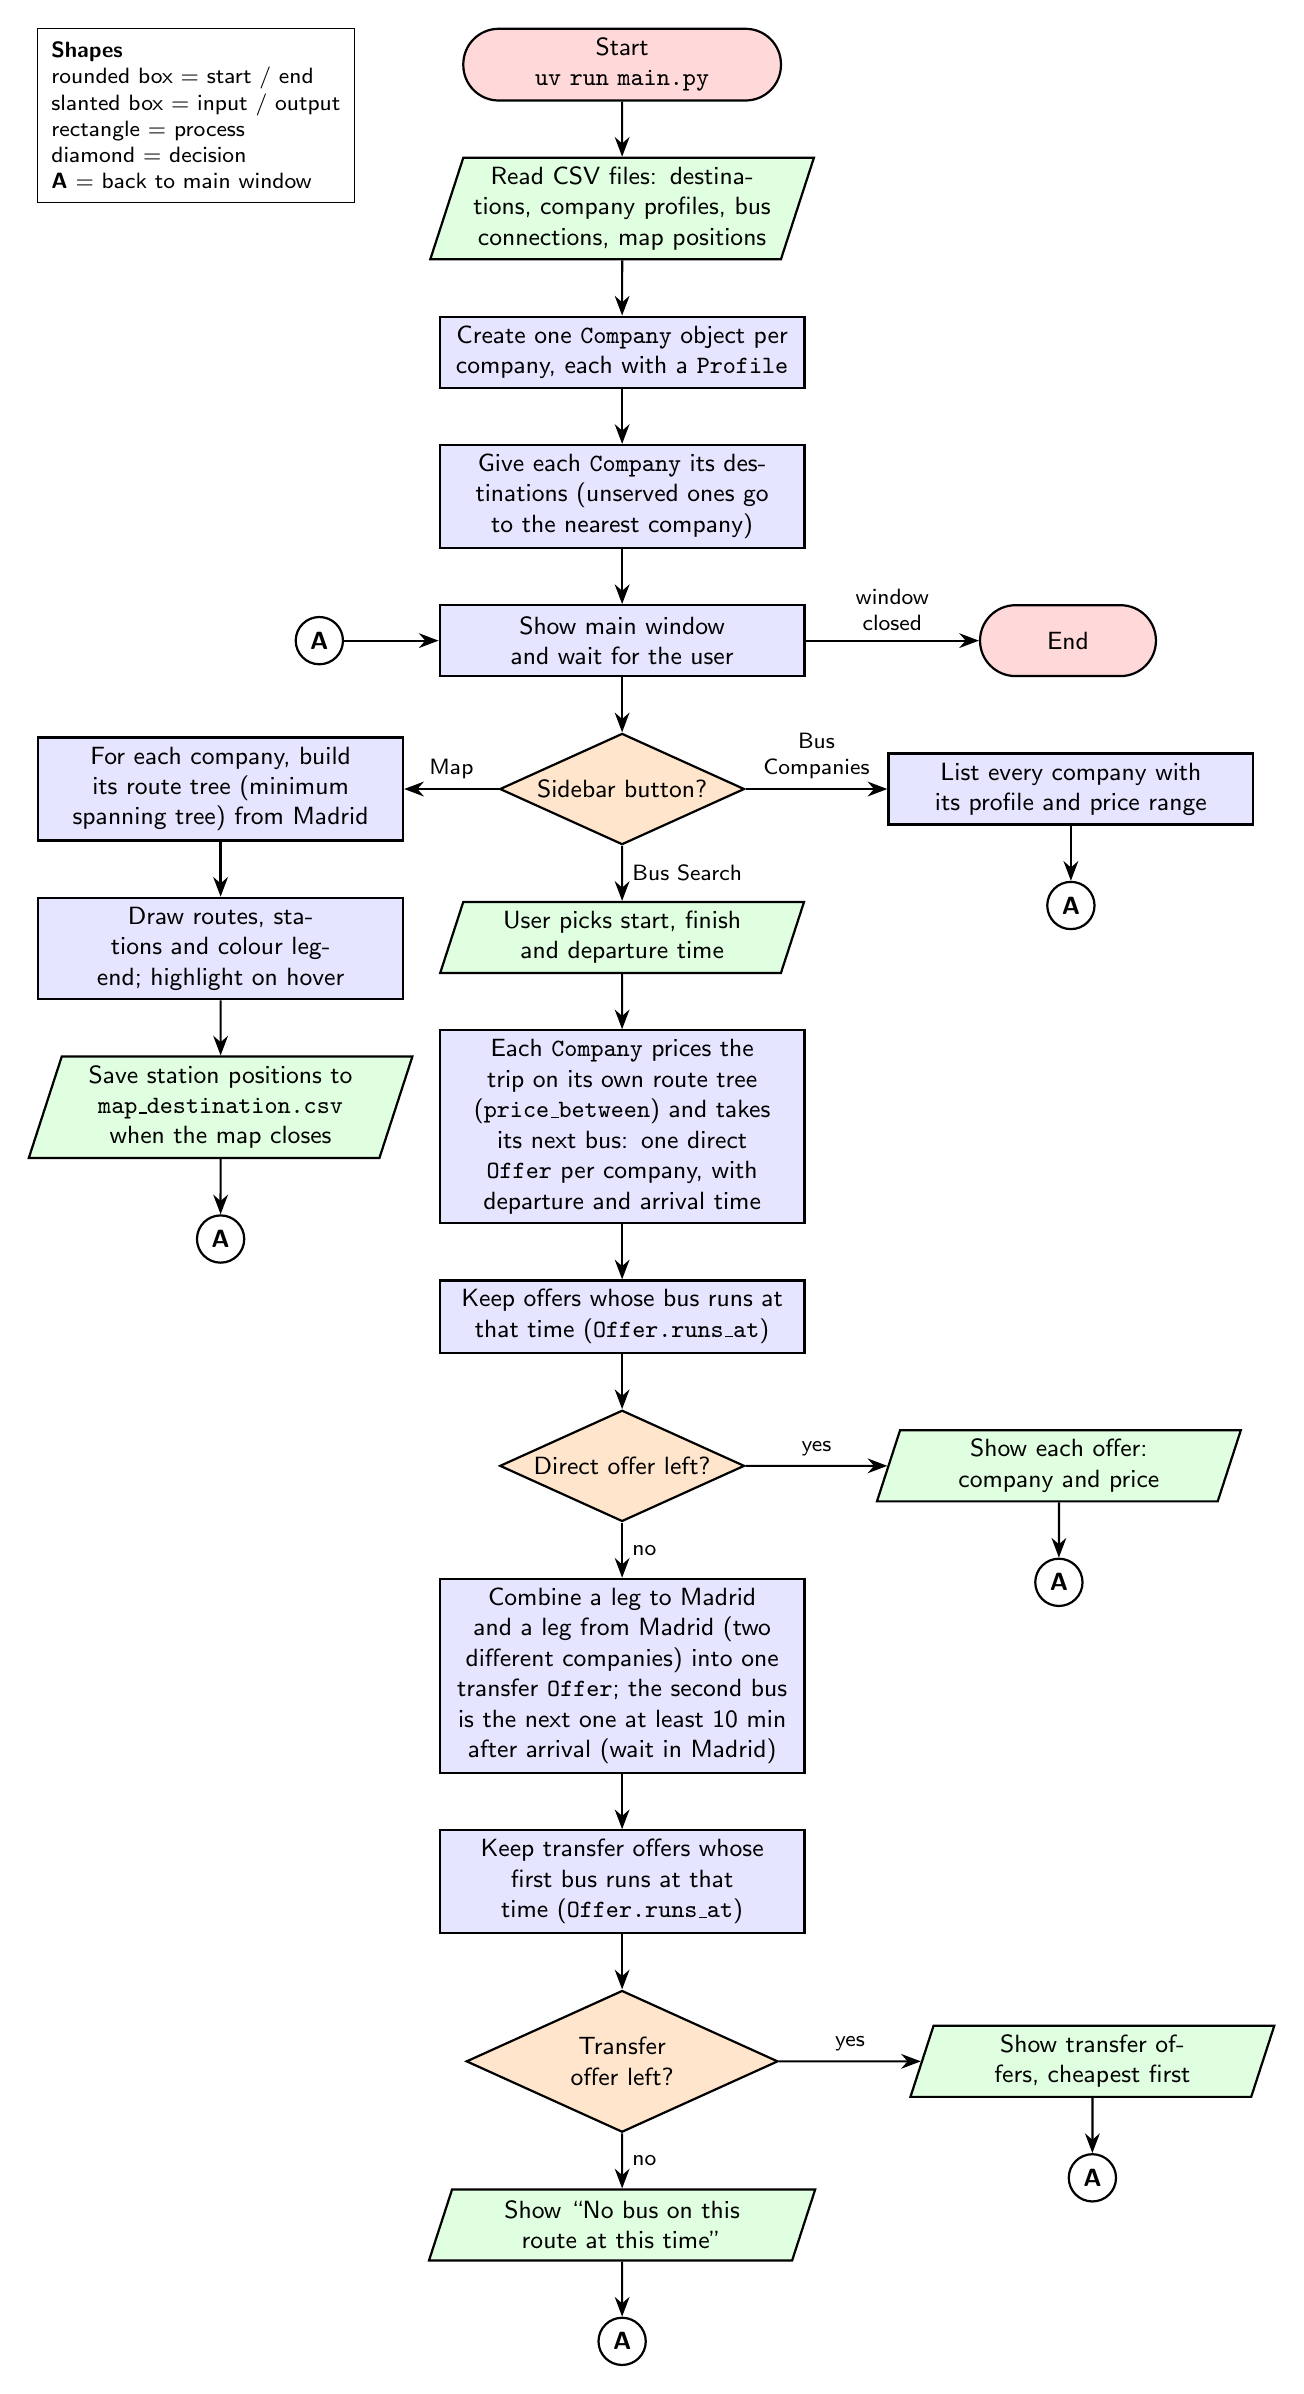
\begin{tikzpicture}[node distance=7mm and 12mm]

  % ---------------- Startup: load data and create objects ----------------
  \node[startstop] (start) {Start\\ \texttt{uv run main.py}};
  \node[io, below=of start] (csv)
    {Read CSV files: destinations, company profiles, bus connections, map positions};
  \node[process, below=of csv] (objects)
    {Create one \texttt{Company} object per company, each with a \texttt{Profile}};
  \node[process, below=of objects] (assign)
    {Give each \texttt{Company} its destinations (unserved ones go to the nearest company)};
  \node[process, below=of assign] (wait) {Show main window and wait for the user};
  \node[startstop, right=22mm of wait, text width=2cm] (stop) {End};
  \node[connector, left=of wait] (back) {A};
  \node[decision, below=of wait] (choice) {Sidebar button?};

  % ---------------- Map branch (left) ----------------
  \node[process, left=of choice] (map1)
    {For each company, build its route tree (minimum spanning tree) from Madrid};
  \node[process, below=of map1] (map2)
    {Draw routes, stations and colour legend; highlight on hover};
  \node[io, below=of map2] (map3)
    {Save station positions to \texttt{map\_destination.csv} when the map closes};
  \node[connector, below=of map3] (backmap) {A};

  % ---------------- Bus Companies branch (right) ----------------
  \node[process, right=18mm of choice] (comp)
    {List every company with its profile and price range};
  \node[connector, below=of comp] (backcomp) {A};

  % ---------------- Bus Search branch (centre) ----------------
  \node[io, below=of choice] (input) {User picks start, finish and departure time};
  \node[process, below=of input] (price)
    {Each \texttt{Company} prices the trip on its own route tree (\texttt{price\_between}) and takes its next bus: one direct \texttt{Offer} per company, with departure and arrival time};
  \node[process, below=of price] (filter1)
    {Keep offers whose bus runs at that time (\texttt{Offer.runs\_at})};
  \node[decision, below=of filter1] (direct) {Direct offer left?};
  \node[io, right=18mm of direct] (show1) {Show each offer: company and price};
  \node[connector, below=of show1] (back1) {A};
  \node[process, below=of direct] (transfer)
    {Combine a leg to Madrid and a leg from Madrid (two different companies) into one transfer \texttt{Offer}; the second bus is the next one at least 10 min after arrival (wait in Madrid)};
  \node[process, below=of transfer] (filter2)
    {Keep transfer offers whose first bus runs at that time (\texttt{Offer.runs\_at})};
  \node[decision, below=of filter2] (anytransfer) {Transfer offer left?};
  \node[io, right=18mm of anytransfer] (show2) {Show transfer offers, cheapest first};
  \node[connector, below=of show2] (back2) {A};
  \node[io, below=of anytransfer] (show3) {Show ``No bus on this route at this time''};
  \node[connector, below=of show3] (back3) {A};

  % ---------------- Legend (top left) ----------------
  \node[draw, thin, lbl, align=left, anchor=north west, inner sep=5pt] at (map1.west |- start.north)
    {\textbf{Shapes}\\
     rounded box = start / end\\
     slanted box = input / output\\
     rectangle = process\\
     diamond = decision\\
     \textbf{A} = back to main window};

  % ---------------- Arrows ----------------
  \draw[arrow] (start) -- (csv);
  \draw[arrow] (csv) -- (objects);
  \draw[arrow] (objects) -- (assign);
  \draw[arrow] (assign) -- (wait);
  \draw[arrow] (back) -- (wait);
  \draw[arrow] (wait) -- node[lbl, above, align=center] {window\\closed} (stop);
  \draw[arrow] (wait) -- (choice);

  \draw[arrow] (choice) -- node[lbl, above] {Map} (map1);
  \draw[arrow] (map1) -- (map2);
  \draw[arrow] (map2) -- (map3);
  \draw[arrow] (map3) -- (backmap);

  \draw[arrow] (choice) -- node[lbl, above, align=center] {Bus\\Companies} (comp);
  \draw[arrow] (comp) -- (backcomp);

  \draw[arrow] (choice) -- node[lbl, right] {Bus Search} (input);
  \draw[arrow] (input) -- (price);
  \draw[arrow] (price) -- (filter1);
  \draw[arrow] (filter1) -- (direct);
  \draw[arrow] (direct) -- node[lbl, above] {yes} (show1);
  \draw[arrow] (show1) -- (back1);
  \draw[arrow] (direct) -- node[lbl, right] {no} (transfer);
  \draw[arrow] (transfer) -- (filter2);
  \draw[arrow] (filter2) -- (anytransfer);
  \draw[arrow] (anytransfer) -- node[lbl, above] {yes} (show2);
  \draw[arrow] (show2) -- (back2);
  \draw[arrow] (anytransfer) -- node[lbl, right] {no} (show3);
  \draw[arrow] (show3) -- (back3);

\end{tikzpicture}
\end{document}
